\renewcommand{\baselinestretch}{1.2}
\usefonttheme[onlymath]{serif}
\title[Market Power and Contagion]{Market Power and Contagion in Interbank Networks}
\subtitle{An Agent-Based Model of Systemic Risk}

\author{Héctor~Castillo~Andreu}

\institute{
   Departament d'Economia\\
  Universitat Jaume~I
}

\date{19 June 2026}

\subject{Analysis through Agent-Based Models (ABM)}

\pgfdeclareimage[height=.4cm]{university-logo}{img/uji}
\logo{\pgfuseimage{university-logo}}

\AtBeginSection[]
{
  \begin{frame}<beamer>
    \frametitle{Outline}
    \tableofcontents[currentsection]
  \end{frame}
}

\newcommand{\photo}[2][.85]{%
  \begin{center}
    \includegraphics[width=#1\linewidth]{img/#2}
  \end{center}
}

\newcounter{slidenumber}
\newcommand{\frametitlecont}[1]{%
  \frametitle{#1 (\roman{slidenumber})}%
}

%======================================================================
\begin{document}

\setbeamertemplate{footline}{%
  \leavevmode%
  \hbox{%
  \begin{beamercolorbox}[wd=.5\paperwidth,ht=2.5ex,dp=1.125ex,leftskip=.3cm plus1fil,rightskip=.3cm]{author in head/foot}%
    \usebeamerfont{author in head/foot}\insertshortauthor
  \end{beamercolorbox}%
  \begin{beamercolorbox}[wd=.5\paperwidth,ht=2.5ex,dp=1.125ex,leftskip=.3cm,rightskip=.3cm plus1fil]{title in head/foot}%
    \usebeamerfont{title in head/foot}\insertframenumber\,/\,\inserttotalframenumber\ -- \insertshorttitle
  \end{beamercolorbox}}%
  \vskip0pt%
}

\begin{frame}
  \titlepage
\end{frame}

\begin{frame}<handout>[t,allowframebreaks]
  \frametitle{Outline}
  \tableofcontents
\end{frame}

%======================================================================
\section{Abstract}\label{sec:1}
%======================================================================

\begin{frame}{Abstract: ABM, Interbank Market, and Contagion}
  \begin{itemize}
    \item \textbf{Agent-Based Models} to study systemic risk in interbank credit networks.
    \item Relationship between \textbf{network connectivity}, \textbf{market power}, and \textbf{bankruptcy cascades}.    
    \item \textbf{Non-monotonic trade-off} between risk sharing and systemic risk---connectivity diversifies risk in normal times but amplifies contagion during crises.
    \item The 2008 financial crisis illustrates how risk-sharing mechanisms can fail under high leverage and heterogeneous agents.
  \end{itemize}
\end{frame}

%======================================================================
\section{Risk and Connectivity}\label{sec:2}
%======================================================================

\begin{frame}{The 2008 Crisis: Background}
  \begin{itemize}
    \item Increased bank leverage and corporate debt-equity ratios made the economy fragile.
    \item Traditional theory does not fully account for complex agent interactions during crises.
    \item The interbank market became a \textbf{contagion vector}: failure of one bank triggers a domino effect through interlocking exposures.
  \end{itemize}
\end{frame}

\begin{frame}{The Risk-Sharing Trade-off}
  Two opposing effects of network connectivity:
  \begin{itemize}
    \item \textbf{Benefit:} Increasing connectivity allows \textbf{risk sharing}---banks diversify exposure across more counterparties.
    \item \textbf{Cost:} Excessive connectivity increases \textbf{systemic risk}---default propagates through the network.
    \item Evidence: a \textbf{non-monotonic relationship} exists---low connectivity stabilizes by diluting shocks, but high connectivity facilitates cascading failures.
  \end{itemize}
  %\vspace{0.3cm}
  %``Spreading the risk around the globe may improve stability in good times. However, in times of crisis, critical perturbations can spread across the whole system.'' -- Tedeschi et al.
\end{frame}

% \begin{frame}{Empirical Evidence}
%   \begin{itemize}
%     \item Allen \& Gale (2000), Thurner et al. (2003), Iori et al. (2006): modeling credit systems as random graphs shows that bankruptcy avalanche probability \textbf{decreases} with connectivity.
%     \item Lorenz \& Battiston (2008) show that with \textbf{financial acceleration} (trend reinforcement in fragility), the probability of default does \textbf{not} decrease monotonically with connectivity.
%     \item Iori et al. (2006) identify \textbf{agent heterogeneity} as the root cause of bankruptcy avalanches.
%     %\item Financial crises are characterized by the \textbf{procyclicality of leverage} across institutions.
%     %\item Reserve requirements dampen cascades but \textbf{limit growth} by reducing firm investment.
%   \end{itemize}
% \end{frame}

\begin{frame}{Channels of Contagion in Financial Crises}
  Three primary propagation mechanisms of systemic failure:
  \begin{enumerate}
    \item \textbf{Bank runs:} self-fulfilling panics where depositors withdraw mass funds simultaneously.
    \item \textbf{Asset price contagion:} fire-sale spirals that depreciate assets across the system.
    \item \textbf{Inter-locking exposures:} direct linkages through the interbank market---default of one bank triggers defaults in connected banks.
  \end{enumerate}
  \vspace{0.3cm}
  Model exposes that through \textbf{rationing} (borrower cannot secure sufficient funding), \textbf{contagion} (lender suffers losses from borrower default), and \textbf{repayment failure}.
\end{frame}


\begin{frame}{Bankruptcies exposed by the model}
  \begin{columns}[T]
    \begin{column}{0.55\textwidth}
      \centering
      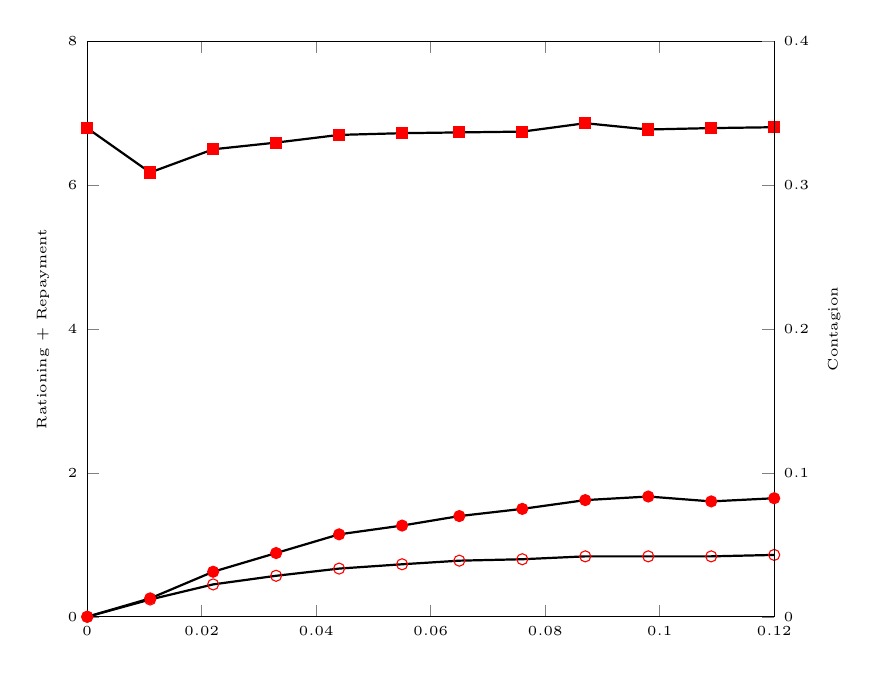
\begin{tikzpicture}
        \begin{axis}[
          width=0.85\textwidth,
          ylabel={Rationing + Repayment},
          ylabel style={font=\tiny},
          ymin=0, ymax=8,
          xmin=0, xmax=0.12,
          xticklabel style={/pgf/number format/fixed, /pgf/number format/precision=2},
          font=\tiny,
        ]
          \addplot[only marks, mark=square*, red] coordinates {
            (0.00001,6.7931)            (0.01100,6.1768)            (0.02200,6.4994)            (0.03300,6.5926)            (0.04400,6.6995)            (0.05500,6.7234)            (0.06500,6.7342)            (0.07600,6.7453)            (0.08700,6.8621)            (0.09800,6.7748)            (0.10900,6.7942)            (0.12000,6.8065)
          };
          \addplot[black, thick]coordinates {
            (0.00001,6.7931)            (0.01100,6.1768)            (0.02200,6.4994)            (0.03300,6.5926)            (0.04400,6.6995)            (0.05500,6.7234)            (0.06500,6.7342)            (0.07600,6.7453)            (0.08700,6.8621)            (0.09800,6.7748)            (0.10900,6.7942)            (0.12000,6.8065)
          };
          \addplot[only marks, mark=o, red] coordinates {
            (0.00001,0.00)            (0.01100,0.24)            (0.02200,0.45)            (0.03300,0.57)            (0.04400,0.67)            (0.05500,0.73)            (0.06500,0.78)            (0.07600,0.80)            (0.08700,0.84)            (0.09800,0.84)            (0.10900,0.84)            (0.12000,0.86)
          };
          \addplot[black, thick]coordinates {
            (0.00001,0.00)            (0.01100,0.24)            (0.02200,0.45)            (0.03300,0.57)            (0.04400,0.67)            (0.05500,0.73)            (0.06500,0.78)            (0.07600,0.80)            (0.08700,0.84)            (0.09800,0.84)            (0.10900,0.84)            (0.12000,0.86)
          };
        \end{axis}
        \begin{axis}[
          width=0.85\textwidth,
          ylabel={Contagion},
          ylabel style={font=\tiny},
          ymin=0, ymax=0.4,
          xmin=0, xmax=0.12,
          axis y line*=right, axis x line=none,
          ylabel near ticks,
          yticklabel style={/pgf/number format/fixed, /pgf/number format/precision=2},
          font=\tiny,
        ]
          \addplot[only marks, mark=*, red] coordinates {
            (0.00001,0.0000)            (0.01100,0.0128)            (0.02200,0.0313)            (0.03300,0.0443)            (0.04400,0.0573)            (0.05500,0.0634)            (0.06500,0.0700)            (0.07600,0.0750)            (0.08700,0.0811)            (0.09800,0.0836)            (0.10900,0.0802)            (0.12000,0.0824)
          };
          \addplot[black, thick]coordinates {
            (0.00001,0.0000)            (0.01100,0.0128)            (0.02200,0.0313)            (0.03300,0.0443)            (0.04400,0.0573)            (0.05500,0.0634)            (0.06500,0.0700)            (0.07600,0.0750)            (0.08700,0.0811)            (0.09800,0.0836)            (0.10900,0.0802)            (0.12000,0.0824)
          };
        \end{axis}
        \end{tikzpicture}
    \end{column}
    \begin{column}{0.43\textwidth}
      \tiny
      \begin{minipage}[t]{0.2\textwidth}
        $\square$ Rat.\par
        $\bullet$ Cont.\par
        $\circ$ Fail.
      \end{minipage}
      \begin{minipage}[t]{0.78\textwidth}
        \renewcommand{\arraystretch}{0.55}\setlength{\tabcolsep}{1.5pt}
        \begin{tabular}{lccc}
          \toprule
          $p$ & Rat. & Cont. & Fail. \\
          \midrule
          0.00001 & 6.79 & 0.00 & 0.00 \\
          0.011 & 6.18 & 0.01 & 0.24 \\
          0.022 & 6.50 & 0.03 & 0.45 \\
          0.033 & 6.59 & 0.04 & 0.57 \\
          0.044 & 6.70 & 0.06 & 0.67 \\
          \textbf{0.055} & \textbf{6.72} & \textbf{0.06} & \textbf{0.73} \\
          0.065 & 6.73 & 0.07 & 0.78 \\
          0.076 & 6.75 & 0.07 & 0.80 \\
          0.087 & 6.86 & 0.08 & 0.84 \\
          0.098 & 6.77 & 0.08 & 0.84 \\
          0.109 & 6.79 & 0.08 & 0.84 \\
          0.120 & 6.81 & 0.08 & 0.86 \\
          \bottomrule
        \end{tabular}
      \end{minipage}
    \end{column}
  \end{columns}
  \vspace{0.3cm}

  {\tiny
  Initial conditions for each bank:
  \begin{tabular}{l|l}
    \multicolumn{1}{c|}{\textbf{Assets}} & \multicolumn{1}{c}{\textbf{Liabilities}} \\ \hline
    $C^i_0= 5-0.18 = 4.82$ & $D^i_0= 9$\\
    $L^i_0= 5$ & $E^i_0= 1$ \\
    $R^i_0 = 0.18$ &
  \end{tabular} \\
  Monte Carlo simulations with $\mathit{MC} = 30$ runs, $N=50$ banks, $T=1000$ periods, and $p$ varying from 0 to 0.12 in increments of 0.01.
  }
\end{frame}



%======================================================================
\section{Model Framework}\label{sec:3}
%======================================================================

\begin{frame}{Model Overview}
  \begin{itemize}
    \item ABM with $N$ banks in a sequential economy $t = \{0, 1, \dots, T\}$.
    \item Banks connected through an \textbf{Erd\H{o}s--R\'enyi} random graph $G(N, p)$: each edge exists with probability $p$.
    \item Three interacting sectors: goods market, credit market, interbank market.
    \item Goal: analyze how \textbf{connectivity} and \textbf{market power} affect system stability.
  \end{itemize}
\end{frame}

\begin{frame}{Balance Sheet}
  \begin{block}{Accounting Identity}
    $L_i^t + C_i^t + R_i^t = D_i^t + E_i^t$
  \end{block}
  \begin{itemize}
    \item \textbf{Assets:} Long-term loans ($L$), liquidity ($C$), reserves ($R$).
    \item \textbf{Liabilities:} Deposits ($D$), equity ($E$).
    \item Reserves set by regulation: $R_i^t = \hat{r} D_i^t$ with $\hat{r} = 0.02$.
  \end{itemize}
\end{frame}

\begin{frame}{Liquidity Shocks}
  Deposits are exogenously shocked each period:
  \[
    D_i^t = D_i^{t-1} [\mu + \omega \cdot U(0,1)]
  \]
  \begin{itemize}
    \item $\mu$: expected growth rate (0.7).
    \item $\omega$: shock magnitude (0.35).
    \item \textbf{Potential lenders:} banks with positive net deposits (after reserves).
    \item \textbf{Potential borrowers:} banks with negative net deposits exceeding liquidity.
  \end{itemize}
\end{frame}

\begin{frame}{Liquidity in the model}
  \begin{columns}[T]
    \begin{column}{0.4\textwidth}
      \centering
      \small $p=[0 .. 1]$\\
      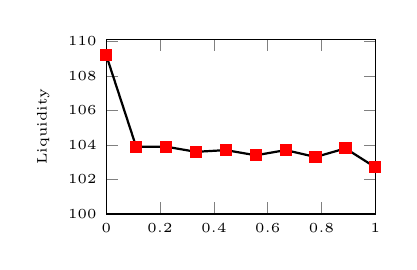
\begin{tikzpicture}
        \begin{axis}[
          ylabel={Liquidity},
          ylabel style={font=\tiny},
          ymin=100,
          xmin=0, xmax=1.0,
          xticklabel style={/pgf/number format/fixed, /pgf/number format/precision=2},
          width=5cm, height=3.8cm,
          font=\tiny,
        ]
          \addplot[only marks, mark=square*, red] coordinates { (1e-05,109.2) (0.11112,103.9) (0.22223,103.9) (0.33334,103.6) (0.44445,103.7) (0.5555599999999999,103.4) (0.66667,103.7) (0.7777799999999999,103.3) (0.88889,103.8) (1.0,102.7) };
          \addplot[black, thick] coordinates { (1e-05,109.2) (0.11112,103.9) (0.22223,103.9) (0.33334,103.6) (0.44445,103.7) (0.5555599999999999,103.4) (0.66667,103.7) (0.7777799999999999,103.3) (0.88889,103.8) (1.0,102.7) };
        \end{axis}
      \end{tikzpicture}
      \vspace{-0.3cm}
      \tiny\renewcommand{\arraystretch}{0.85}\setlength{\tabcolsep}{2pt}
      \centering
      \begin{tabular}{lr}
        \toprule
        $p$ & Val. \\
        \midrule
          0.00001 & 109.2 \\
          0.111 & 103.9 \\
          0.222 & 103.9 \\
          0.333 & 103.6 \\
          0.444 & 103.7 \\
          0.556 & 103.4 \\
          0.667 & 103.7 \\
          0.778 & 103.3 \\
          0.889 & 103.8 \\
          1.000 & 102.7 \\
        \bottomrule
      \end{tabular}
    \end{column}
    \begin{column}{0.6\textwidth}
      \centering
      \small $p=[0 .. 0.12]$\\
      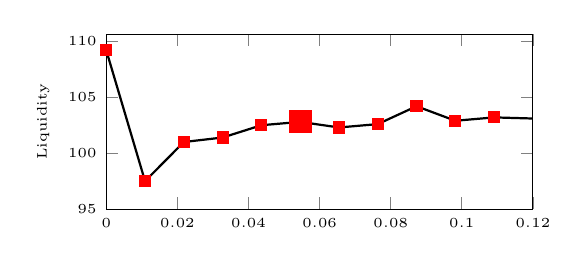
\begin{tikzpicture}
        \begin{axis}[
          ylabel={Liquidity},
          ylabel style={font=\tiny},
          ymin=95,
          xmin=0, xmax=0.12,
          xticklabel style={/pgf/number format/fixed, /pgf/number format/precision=2},
          width=7cm, height=3.8cm,
          font=\tiny,
        ]
          \addplot[only marks, mark=square*, red] coordinates { (1e-05,109.2) (0.01091909090909091,97.5) (0.02182818181818182,101.0) (0.03273727272727273,101.4) (0.04364636363636364,102.5) (0.05455545454545455,102.8) (0.06546454545454546,102.3) (0.07637363636363637,102.6) (0.08728272727272728,104.2) (0.09819181818181819,102.9) (0.1091009090909091,103.2) (0.12001,103.1) };
          \addplot[black, thick] coordinates { (1e-05,109.2) (0.01091909090909091,97.5) (0.02182818181818182,101.0) (0.03273727272727273,101.4) (0.04364636363636364,102.5) (0.05455545454545455,102.8) (0.06546454545454546,102.3) (0.07637363636363637,102.6) (0.08728272727272728,104.2) (0.09819181818181819,102.9) (0.1091009090909091,103.2) (0.12001,103.1) };
          \addplot[only marks, mark=square*, red, mark size=4] coordinates { (0.05455545454545455,102.8) };
        \end{axis}
      \end{tikzpicture}
      \vspace{-0.3cm}
      \tiny\renewcommand{\arraystretch}{0.85}\setlength{\tabcolsep}{2pt}
      \centering
      \begin{tabular}{lr}
        \toprule
        $p$ & Val. \\
        \midrule
          0.00001 & 109.2 \\
          0.011 & 97.5 \\
          0.022 & 101.0 \\
          0.033 & 101.4 \\
          0.044 & 102.5 \\
          \textbf{0.055} & \textbf{102.8} \\
          0.065 & 102.3 \\
          0.076 & 102.6 \\
          0.087 & 104.2 \\
          0.098 & 102.9 \\
          0.109 & 103.2 \\
          0.120 & 103.1 \\
        \bottomrule
      \end{tabular}
    \end{column}
  \end{columns}
\end{frame}

\begin{frame}{Deposits in the model}
  \begin{columns}[T]
    \begin{column}{0.4\textwidth}
      \centering
      \small $p=[0 .. 1]$\\
      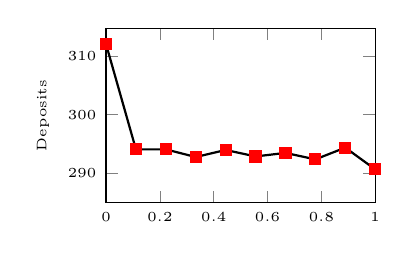
\begin{tikzpicture}
        \begin{axis}[
          ylabel={Deposits},
          ylabel style={font=\tiny},
          ymin=285,
          xmin=0, xmax=1.0,
          xticklabel style={/pgf/number format/fixed, /pgf/number format/precision=2},
          width=5cm, height=3.8cm,
          font=\tiny,
        ]
          \addplot[only marks, mark=square*, red] coordinates { (1e-05,312.0) (0.11112,294.1) (0.22223,294.1) (0.33334,292.8) (0.44445,294.0) (0.5555599999999999,292.9) (0.66667,293.5) (0.7777799999999999,292.4) (0.88889,294.4) (1.0,290.7) };
          \addplot[black, thick] coordinates { (1e-05,312.0) (0.11112,294.1) (0.22223,294.1) (0.33334,292.8) (0.44445,294.0) (0.5555599999999999,292.9) (0.66667,293.5) (0.7777799999999999,292.4) (0.88889,294.4) (1.0,290.7) };
        \end{axis}
      \end{tikzpicture}
      \vspace{-0.3cm}
      \tiny\renewcommand{\arraystretch}{0.85}\setlength{\tabcolsep}{2pt}
      \centering
      \begin{tabular}{lr}
        \toprule
        $p$ & Val. \\
        \midrule
          0.00001 & 312.0 \\
          0.111 & 294.1 \\
          0.222 & 294.1 \\
          0.333 & 292.8 \\
          0.444 & 294.0 \\
          0.556 & 292.9 \\
          0.667 & 293.5 \\
          0.778 & 292.4 \\
          0.889 & 294.4 \\
          1.000 & 290.7 \\
        \bottomrule
      \end{tabular}
    \end{column}
    \begin{column}{0.6\textwidth}
      \centering
      \small $p=[0 .. 0.12]$\\
      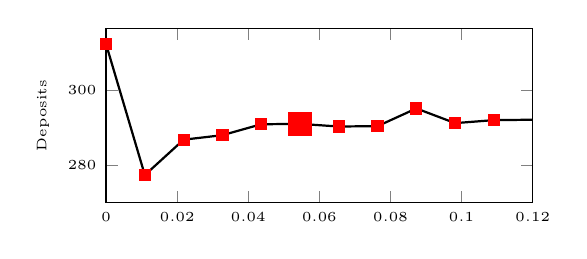
\begin{tikzpicture}
        \begin{axis}[
          ylabel={Deposits},
          ylabel style={font=\tiny},
          ymin=270,
          xmin=0, xmax=0.12,
          xticklabel style={/pgf/number format/fixed, /pgf/number format/precision=2},
          width=7cm, height=3.8cm,
          font=\tiny,
        ]
          \addplot[only marks, mark=square*, red] coordinates { (1e-05,312.2) (0.01091909090909091,277.4) (0.02182818181818182,286.8) (0.03273727272727273,288.0) (0.04364636363636364,290.9) (0.05455545454545455,291.0) (0.06546454545454546,290.3) (0.07637363636363637,290.4) (0.08728272727272728,295.1) (0.09819181818181819,291.2) (0.1091009090909091,292.0) (0.12001,292.1) };
          \addplot[black, thick] coordinates { (1e-05,312.2) (0.01091909090909091,277.4) (0.02182818181818182,286.8) (0.03273727272727273,288.0) (0.04364636363636364,290.9) (0.05455545454545455,291.0) (0.06546454545454546,290.3) (0.07637363636363637,290.4) (0.08728272727272728,295.1) (0.09819181818181819,291.2) (0.1091009090909091,292.0) (0.12001,292.1) };
          \addplot[only marks, mark=square*, red, mark size=4] coordinates { (0.05455545454545455,291.0) };
        \end{axis}
      \end{tikzpicture}
      \vspace{-0.3cm}
      \tiny\renewcommand{\arraystretch}{0.85}\setlength{\tabcolsep}{2pt}
      \centering
      \begin{tabular}{lr}
        \toprule
        $p$ & Val. \\
        \midrule
          0.00001 & 312.2 \\
          0.011 & 277.4 \\
          0.022 & 286.8 \\
          0.033 & 288.0 \\
          0.044 & 290.9 \\
          \textbf{0.055} & \textbf{291.0} \\
          0.065 & 290.3 \\
          0.076 & 290.4 \\
          0.087 & 295.1 \\
          0.098 & 291.2 \\
          0.109 & 292.0 \\
          0.120 & 292.1 \\
        \bottomrule
      \end{tabular}
    \end{column}
  \end{columns}
\end{frame}

\begin{frame}{Network Structure}
  \begin{itemize}
    \item Bilateral credit lines formed at the start of each period.
    \item Connectivity controlled by parameter $p$ in the Erd\H{o}s--R\'enyi graph.
    \item Each borrower is matched to \textbf{exactly one} lender per period.
    \item The \textbf{Giant Component Size (GCS)} measures network integration.
  \end{itemize}
\end{frame}

{\usebackgroundtemplate{%
  \vbox to 0pt{\vskip40pt\hbox{\hskip30pt
\includegraphics[width=0.9\paperwidth,height=0.85\paperheight,keepaspectratio]{with_directions.png}}\vss}%
}
\begin{frame}[t]
  \frametitle{Erd\H{o}s--R\'enyi Random Graph}
  \vspace{0.5cm}
  \begin{minipage}{0.85\textwidth}
    \vspace{3.5cm}

    \centering
    \footnotesize
    Each of the $\binom{N}{2}$ possible edges is included independently with probability $p$. For $N=50$ banks:
    \begin{itemize}
      \item $p = 0$: isolated banks, no interbank market.
      \item $p = 1/N = 0.02$: \textbf{percolation threshold}---giant component emerges.
      \item $p > 0.05$: network is saturated ($>92\%$ of banks connected).
    \end{itemize}
  \end{minipage}
\end{frame}
}



\begin{frame}{Network Structure}
The Erd\H{o}s--R\'enyi model does not attempt to replicate the entire interbank market; rather, it illustrates how connection density alters the probability and scale of contagion.
\end{frame}


%======================================================================
\section{Interest Rate and Market Power}\label{sec:4}
%======================================================================

\begin{frame}[shrink=0.1]{Law of Supply and Demand}
  \begin{columns}[T]
    \begin{column}{0.52\textwidth}
      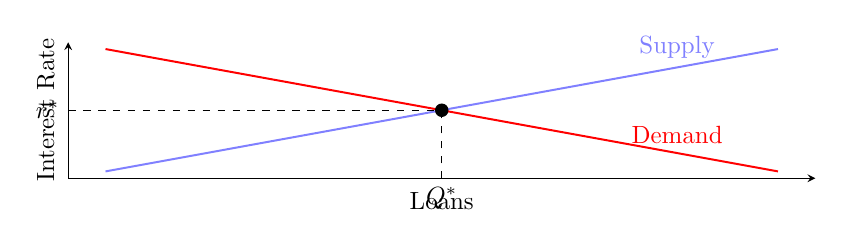
\begin{tikzpicture}[scale=0.9]
          \begin{axis}[
            xmin=0, xmax=10, ymin=0, ymax=10,
            xlabel={Loans},
            ylabel={Interest Rate},
            axis lines=left,
            xtick=\empty, ytick=\empty,
            clip=false,
            width=\textwidth,
            height=3.5cm,
          ]
          \addplot[blue!50!white, thick, domain=0.5:9.5] {x} node[pos=0.85, above, blue!50!white] {Supply};
          \addplot[red, thick, domain=0.5:9.5] {10 - x} node[pos=0.85, above, red] {Demand};
          \draw[dashed] (axis cs:5,0) -- (axis cs:5,5) node[pos=0, below] {$Q^*$};
          \draw[dashed] (0,5) -- (axis cs:5,5) node[pos=0, left] {$r^*$};
          \draw[fill=black] (axis cs:5,5) circle (2.5pt) node[above right] {};
          \end{axis}
        \end{tikzpicture}
    \end{column}
    \begin{column}{0.45\textwidth}
      \small
      Model manages \textbf{market power} as a parameter $\psi$, which correlates with bank size and reflects the capacity to influence market terms, respecting the law of supply and demand.
%      \begin{itemize}
%        \item \textcolor{blue}{\textbf{Supply}} (lenders): more banks willing to lend as interest rate rises / less market power.
%        \item \textcolor{red}{\textbf{Demand}} (borrowers): fewer banks seek credit as interest rate rises / market power grows.
%      \end{itemize}
    \end{column}
  \end{columns}

  \vspace{0.15cm}
  \begin{columns}[T]
    \begin{column}{0.48\textwidth}
      \centering
      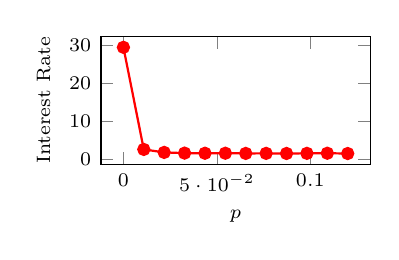
\begin{tikzpicture}
        \begin{axis}[
          width=5cm, height=3.2cm,
          xlabel={$p$},
          ylabel={Interest Rate},
          font=\scriptsize,
        ]
        \addplot[red, thick, mark=*] coordinates {
          (0.00001, 29.5624)
          (0.01092, 2.7021)
          (0.02183, 1.9175)
          (0.03274, 1.7330)
          (0.04365, 1.6967)
          (0.05456, 1.7014)
          (0.06546, 1.6538)
          (0.07637, 1.6649)
          (0.08728, 1.6399)
          (0.09819, 1.6700)
          (0.10910, 1.7010)
          (0.12001, 1.6250)
        };
        \end{axis}
      \end{tikzpicture}
    \end{column}
    \begin{column}{0.48\textwidth}
      \centering
      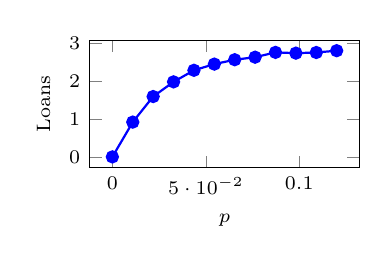
\begin{tikzpicture}
        \begin{axis}[
          width=5cm, height=3.2cm,
          xlabel={$p$},
          ylabel={Loans},
          font=\scriptsize,
        ]
        \addplot[blue, thick, mark=*] coordinates {
          (0.00001, 0.0015)
          (0.01092, 0.9186)
          (0.02183, 1.5923)
          (0.03274, 1.9792)
          (0.04365, 2.2841)
          (0.05456, 2.4472)
          (0.06546, 2.5627)
          (0.07637, 2.6294)
          (0.08728, 2.7562)
          (0.09819, 2.7360)
          (0.10910, 2.7532)
          (0.12001, 2.8009)
        };
        \end{axis}
      \end{tikzpicture}
    \end{column}
  \end{columns}
\end{frame}

\begin{frame}{Expected Profit}
  Banks are risk-neutral in perfect competition. Expected profit from lending to borrower $j$:
  \begin{block}{}
    $E[\Pi_{i,j}^t] = p_j^t (r_{i,j}^t - m) c_{i,j}^t - (1 - p_j^t) m \cdot c_{i,j}^t$
  \end{block}
  \begin{itemize}
    \item $m$: screening cost ($0.015$).
    \item $p_j^t$: probability of borrower survival.
    \item $r_{i,j}^t$: interest rate; $c_{i,j}^t$: lending capacity.
  \end{itemize}
\end{frame}

\begin{frame}{Interest Rate Derivation}
  Setting $E[\Pi] = 0$ (zero-profit condition):
  \[
    r_{i,j}^t = \frac{m}{p_j^t}
  \]
  Introducing \textbf{market power} $\psi \in [0,1)$:
  \[
    \boxed{r_{i,j}^t = \frac{m}{p_j^t (1 - \psi)}}
  \]
  \begin{itemize}
    \item $\psi = 0$: competitive (actuarially fair) rate.
    \item $\psi > 0$: monopolistic markup from information asymmetry.
  \end{itemize}
\end{frame}


\begin{frame}{Interest Rate in the model}
  \begin{columns}[T]
    \begin{column}{0.4\textwidth}
      \centering
      \small $p=[0 .. 1]$\\
      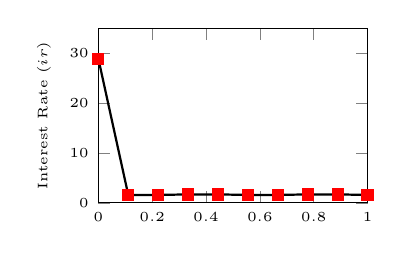
\begin{tikzpicture}
        \begin{axis}[
          ylabel={Interest Rate ($ir$)},
          ylabel style={font=\tiny},
          ymin=0, ymax=35,
          xmin=0, xmax=1.0,
          xticklabel style={/pgf/number format/fixed, /pgf/number format/precision=2},
          width=5cm, height=3.8cm,
          font=\tiny,
        ]
          \addplot[only marks, mark=square*, red] coordinates { (1e-05,28.9) (0.11112,1.6) (0.22223,1.6) (0.33334,1.7) (0.44445,1.7) (0.5555599999999999,1.6) (0.66667,1.6) (0.7777799999999999,1.7) (0.88889,1.7) (1.0,1.6) };
          \addplot[black, thick] coordinates { (1e-05,28.9) (0.11112,1.6) (0.22223,1.6) (0.33334,1.7) (0.44445,1.7) (0.5555599999999999,1.6) (0.66667,1.6) (0.7777799999999999,1.7) (0.88889,1.7) (1.0,1.6) };
        \end{axis}
      \end{tikzpicture}
      \vspace{-0.3cm}
      \tiny\renewcommand{\arraystretch}{0.85}\setlength{\tabcolsep}{2pt}
      \centering
      \begin{tabular}{lr}
        \toprule
        $p$ & Val. \\
        \midrule
          0.00001 & 28.9 \\
          0.111 & 1.6 \\
          0.222 & 1.6 \\
          0.333 & 1.7 \\
          0.444 & 1.7 \\
          0.556 & 1.6 \\
          0.667 & 1.6 \\
          0.778 & 1.7 \\
          0.889 & 1.7 \\
          1.000 & 1.6 \\
        \bottomrule
      \end{tabular}
    \end{column}
    \begin{column}{0.6\textwidth}
      \centering
      \small $p=[0 .. 0.12]$\\
      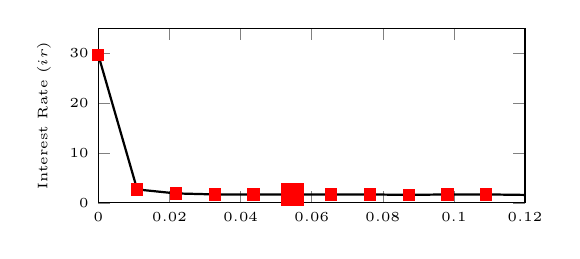
\begin{tikzpicture}
        \begin{axis}[
          ylabel={Interest Rate ($ir$)},
          ylabel style={font=\tiny},
          ymin=0, ymax=35,
          xmin=0, xmax=0.12,
          xticklabel style={/pgf/number format/fixed, /pgf/number format/precision=2},
          width=7cm, height=3.8cm,
          font=\tiny,
        ]
          \addplot[only marks, mark=square*, red] coordinates { (1e-05,29.6) (0.01091909090909091,2.7) (0.02182818181818182,1.9) (0.03273727272727273,1.7) (0.04364636363636364,1.7) (0.05455545454545455,1.7) (0.06546454545454546,1.7) (0.07637363636363637,1.7) (0.08728272727272728,1.6) (0.09819181818181819,1.7) (0.1091009090909091,1.7) (0.12001,1.6) };
          \addplot[black, thick] coordinates { (1e-05,29.6) (0.01091909090909091,2.7) (0.02182818181818182,1.9) (0.03273727272727273,1.7) (0.04364636363636364,1.7) (0.05455545454545455,1.7) (0.06546454545454546,1.7) (0.07637363636363637,1.7) (0.08728272727272728,1.6) (0.09819181818181819,1.7) (0.1091009090909091,1.7) (0.12001,1.6) };
          \addplot[only marks, mark=square*, red, mark size=4] coordinates { (0.05455545454545455,1.7) };
        \end{axis}
      \end{tikzpicture}
      \vspace{-0.3cm}
      \tiny\renewcommand{\arraystretch}{0.85}\setlength{\tabcolsep}{2pt}
      \centering
      \begin{tabular}{lr}
        \toprule
        $p$ & Val. \\
        \midrule
          0.00001 & 29.6 \\
          0.011 & 2.7 \\
          0.022 & 1.9 \\
          0.033 & 1.7 \\
          0.044 & 1.7 \\
          \textbf{0.055} & \textbf{1.7} \\
          0.065 & 1.7 \\
          0.076 & 1.7 \\
          0.087 & 1.6 \\
          0.098 & 1.7 \\
          0.109 & 1.7 \\
          0.120 & 1.6 \\
        \bottomrule
      \end{tabular}
    \end{column}
  \end{columns}
\end{frame}

\begin{frame}{Endogenous Market Power}
  Market power evolves endogenously with bank size:
  \[
    \psi_i^t = \frac{E_i^t}{E_i^{t,\max}}
  \]
  \begin{itemize}
    \item Larger banks (higher equity) exercise more market power.
    \item Borrower default probability:
    $p_{b,j}^t = E_j^t / E_j^{t,\max}$.
    \item Leverage: $\lambda_j^t = d_j^t / E_j^t$.
    \item The model evolves \textbf{only} from screening costs and shock parameters.
  \end{itemize}
\end{frame}


\begin{frame}{Market Power in the model}
  \begin{columns}[T]
    \begin{column}{0.4\textwidth}
      \centering
      \small $p=[0 .. 1]$\\
      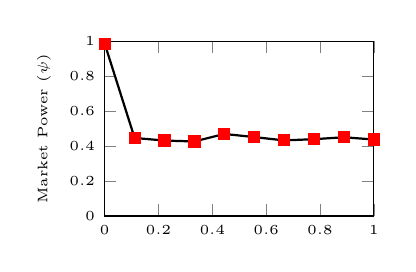
\begin{tikzpicture}
        \begin{axis}[
          ylabel={Market Power ($\psi$)},
          ylabel style={font=\tiny},
          ymin=0, ymax=1,
          xmin=0, xmax=1.0,
          xticklabel style={/pgf/number format/fixed, /pgf/number format/precision=2},
          width=5cm, height=3.8cm,
          font=\tiny,
        ]
          \addplot[only marks, mark=square*, red] coordinates { (1e-05,0.987) (0.11112,0.447) (0.22223,0.432) (0.33334,0.427) (0.44445,0.470) (0.5555599999999999,0.452) (0.66667,0.433) (0.7777799999999999,0.440) (0.88889,0.451) (1.0,0.438) };
          \addplot[black, thick] coordinates { (1e-05,0.987) (0.11112,0.447) (0.22223,0.432) (0.33334,0.427) (0.44445,0.470) (0.5555599999999999,0.452) (0.66667,0.433) (0.7777799999999999,0.440) (0.88889,0.451) (1.0,0.438) };
        \end{axis}
      \end{tikzpicture}
      \vspace{-0.3cm}
      \tiny\renewcommand{\arraystretch}{0.85}\setlength{\tabcolsep}{2pt}
      \centering
      \begin{tabular}{lr}
        \toprule
        $p$ & Val. \\
        \midrule
          0.00001 & 0.987 \\
          0.111 & 0.447 \\
          0.222 & 0.432 \\
          0.333 & 0.427 \\
          0.444 & 0.470 \\
          0.556 & 0.452 \\
          0.667 & 0.433 \\
          0.778 & 0.440 \\
          0.889 & 0.451 \\
          1.000 & 0.438 \\
        \bottomrule
      \end{tabular}
    \end{column}
    \begin{column}{0.6\textwidth}
      \centering
      \small $p=[0 .. 0.12]$\\
      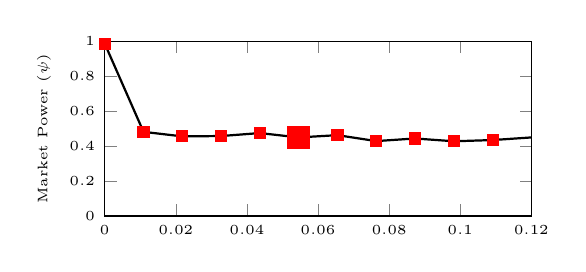
\begin{tikzpicture}
        \begin{axis}[
          ylabel={Market Power ($\psi$)},
          ylabel style={font=\tiny},
          ymin=0, ymax=1,
          xmin=0, xmax=0.12,
          xticklabel style={/pgf/number format/fixed, /pgf/number format/precision=2},
          width=7cm, height=3.8cm,
          font=\tiny,
        ]
          \addplot[only marks, mark=square*, red] coordinates { (1e-05,0.987) (0.01091909090909091,0.482) (0.02182818181818182,0.456) (0.03273727272727273,0.458) (0.04364636363636364,0.475) (0.05455545454545455,0.450) (0.06546454545454546,0.463) (0.07637363636363637,0.429) (0.08728272727272728,0.444) (0.09819181818181819,0.428) (0.1091009090909091,0.435) (0.12001,0.450) };
          \addplot[black, thick] coordinates { (1e-05,0.987) (0.01091909090909091,0.482) (0.02182818181818182,0.456) (0.03273727272727273,0.458) (0.04364636363636364,0.475) (0.05455545454545455,0.450) (0.06546454545454546,0.463) (0.07637363636363637,0.429) (0.08728272727272728,0.444) (0.09819181818181819,0.428) (0.1091009090909091,0.435) (0.12001,0.450) };
          \addplot[only marks, mark=square*, red, mark size=4] coordinates { (0.05455545454545455,0.450) };
        \end{axis}
      \end{tikzpicture}
      \vspace{-0.3cm}
      \tiny\renewcommand{\arraystretch}{0.85}\setlength{\tabcolsep}{2pt}
      \centering
      \begin{tabular}{lr}
        \toprule
        $p$ & Val. \\
        \midrule
          0.00001 & 0.987 \\
          0.011 & 0.482 \\
          0.022 & 0.456 \\
          0.033 & 0.458 \\
          0.044 & 0.475 \\
          \textbf{0.055} & \textbf{0.450} \\
          0.065 & 0.463 \\
          0.076 & 0.429 \\
          0.087 & 0.444 \\
          0.098 & 0.428 \\
          0.109 & 0.435 \\
          0.120 & 0.450 \\
        \bottomrule
      \end{tabular}
    \end{column}
  \end{columns}
\end{frame}

%======================================================================
\section{Equity and Bankruptcy Dynamics}\label{sec:5}
%======================================================================

\begin{frame}{Equity Evolution}
  \[
    E_t^i = E_{t-1}^i + \sum_{j} l_{t}^{i,j} r_{t}^{i,j} - \sum_{j \subseteq \theta_t^i} \left[ B_t^{i,j} - \tilde{L}_t^j \right]
  \]
  \begin{itemize}
    \item \textbf{Bankruptcy:} bank exits if $E_i^t < 0$.
    \item \textbf{Fire sales:} last-resort option (blocked in this model to amplify contagion effects).
    \item Failed banks replaced by new entrants with small initial capital.
  \end{itemize}
\end{frame}


\begin{frame}{Equity in the model}
  \begin{columns}[T]
    \begin{column}{0.4\textwidth}
      \centering
      \small $p=[0 .. 1]$\\
      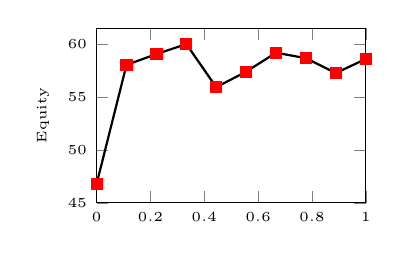
\begin{tikzpicture}
        \begin{axis}[
          ylabel={Equity},
          ylabel style={font=\tiny},
          ymin=45,
          xmin=0, xmax=1.0,
          xticklabel style={/pgf/number format/fixed, /pgf/number format/precision=2},
          width=5cm, height=3.8cm,
          font=\tiny,
        ]
          \addplot[only marks, mark=square*, red] coordinates { (1e-05,46.79) (0.11112,58.01) (0.22223,59.03) (0.33334,59.97) (0.44445,55.91) (0.5555599999999999,57.37) (0.66667,59.16) (0.7777799999999999,58.64) (0.88889,57.24) (1.0,58.57) };
          \addplot[black, thick] coordinates { (1e-05,46.79) (0.11112,58.01) (0.22223,59.03) (0.33334,59.97) (0.44445,55.91) (0.5555599999999999,57.37) (0.66667,59.16) (0.7777799999999999,58.64) (0.88889,57.24) (1.0,58.57) };
        \end{axis}
      \end{tikzpicture}
      \vspace{-0.3cm}
      \tiny\renewcommand{\arraystretch}{0.85}\setlength{\tabcolsep}{2pt}
      \centering
      \begin{tabular}{lr}
        \toprule
        $p$ & Val. \\
        \midrule
          0.00001 & 46.79 \\
          0.111 & 58.01 \\
          0.222 & 59.03 \\
          0.333 & 59.97 \\
          0.444 & 55.91 \\
          0.556 & 57.37 \\
          0.667 & 59.16 \\
          0.778 & 58.64 \\
          0.889 & 57.24 \\
          1.000 & 58.57 \\
        \bottomrule
      \end{tabular}
    \end{column}
    \begin{column}{0.6\textwidth}
      \centering
      \small $p=[0 .. 0.12]$\\
      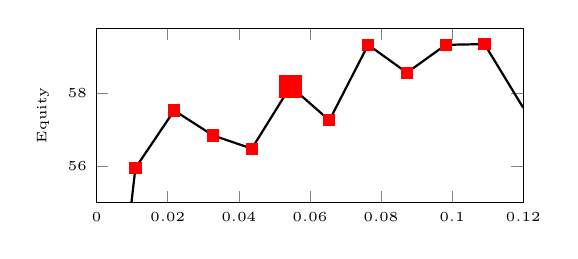
\begin{tikzpicture}
        \begin{axis}[
          ylabel={Equity},
          ylabel style={font=\tiny},
          ymin=55,
          xmin=0, xmax=0.12,
          xticklabel style={/pgf/number format/fixed, /pgf/number format/precision=2},
          width=7cm, height=3.8cm,
          font=\tiny,
        ]
          \addplot[only marks, mark=square*, red] coordinates { (1e-05,46.81) (0.01091909090909091,55.95) (0.02182818181818182,57.52) (0.03273727272727273,56.84) (0.04364636363636364,56.48) (0.05455545454545455,58.18) (0.06546454545454546,57.25) (0.07637363636363637,59.31) (0.08728272727272728,58.55) (0.09819181818181819,59.31) (0.1091009090909091,59.33) (0.12001,57.59) };
          \addplot[black, thick] coordinates { (1e-05,46.81) (0.01091909090909091,55.95) (0.02182818181818182,57.52) (0.03273727272727273,56.84) (0.04364636363636364,56.48) (0.05455545454545455,58.18) (0.06546454545454546,57.25) (0.07637363636363637,59.31) (0.08728272727272728,58.55) (0.09819181818181819,59.31) (0.1091009090909091,59.33) (0.12001,57.59) };
          \addplot[only marks, mark=square*, red, mark size=4] coordinates { (0.05455545454545455,58.18) };
        \end{axis}
      \end{tikzpicture}
      \vspace{-0.3cm}
      \tiny\renewcommand{\arraystretch}{0.85}\setlength{\tabcolsep}{2pt}
      \centering
      \begin{tabular}{lr}
        \toprule
        $p$ & Val. \\
        \midrule
          0.00001 & 46.81 \\
          0.011 & 55.95 \\
          0.022 & 57.52 \\
          0.033 & 56.84 \\
          0.044 & 56.48 \\
          \textbf{0.055} & \textbf{58.18} \\
          0.065 & 57.25 \\
          0.076 & 59.31 \\
          0.087 & 58.55 \\
          0.098 & 59.31 \\
          0.109 & 59.33 \\
          0.120 & 57.59 \\
        \bottomrule
      \end{tabular}
    \end{column}
  \end{columns}
\end{frame}

\begin{frame}{Failure Channels}
  Three distinct causes of bank failure:
  \begin{enumerate}
    \item \textbf{Rationing:} borrower cannot secure sufficient funding.
    \item \textbf{Contagion:} lender suffers losses from borrower default (bad debt).
    \item \textbf{Repayment failure:} fully-funded borrower cannot repay loan or interest.
  \end{enumerate}
  \vspace{0.3cm}
  Key finding: \textbf{repayment failure dominates} at high connectivity, while rationing dominates at low connectivity. Contagion remains minimal ($<5\%$).
\end{frame}



\begin{frame}{Failures}
  \begin{columns}[T]
    \begin{column}{0.4\textwidth}
      \centering
      \tiny $p=[0 .. 1]$\\
      \begin{figure}
        \centering
        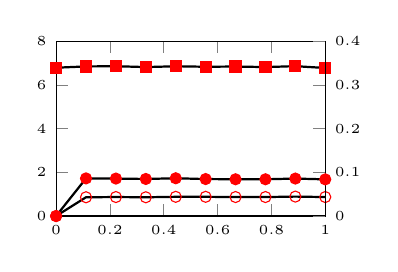
\begin{tikzpicture}
        \begin{axis}[
          %ylabel={Rationing + Repayment},
          ylabel style={font=\tiny, inner sep=0pt, xshift=0pt},
          ymin=0, ymax=8,
          xmin=0, xmax=1.0,
          width=5cm, height=3.8cm,
          font=\tiny,
        ]
          \addplot[only marks, mark=square*, red] coordinates { (1e-05,6.7930) (0.11112,6.8513) (0.22223,6.8612) (0.33334,6.8222) (0.44445,6.8584) (0.5555599999999999,6.8366) (0.66667,6.8472) (0.7777799999999999,6.8218) (0.88889,6.8642) (1.0,6.7793) };
          \addplot[black, thick] coordinates { (1e-05,6.7930) (0.11112,6.8513) (0.22223,6.8612) (0.33334,6.8222) (0.44445,6.8584) (0.5555599999999999,6.8366) (0.66667,6.8472) (0.7777799999999999,6.8218) (0.88889,6.8642) (1.0,6.7793) };
          \addplot[only marks, mark=o, red] coordinates { (1e-05,0.00) (0.11112,0.86) (0.22223,0.87) (0.33334,0.86) (0.44445,0.88) (0.5555599999999999,0.88) (0.66667,0.87) (0.7777799999999999,0.87) (0.88889,0.89) (1.0,0.87) };
          \addplot[black, thick] coordinates { (1e-05,0.00) (0.11112,0.86) (0.22223,0.87) (0.33334,0.86) (0.44445,0.88) (0.5555599999999999,0.88) (0.66667,0.87) (0.7777799999999999,0.87) (0.88889,0.89) (1.0,0.87) };
        \end{axis}
        \begin{axis}[
          %ylabel={Contagion},
          ylabel style={font=\tiny, inner sep=0pt, xshift=-5pt},
          ymin=0, ymax=0.4,
          xmin=0, xmax=1.0,
          axis y line*=right, axis x line=none,
          ylabel near ticks,
          width=5cm, height=3.8cm,
          font=\tiny,
        ]
          \addplot[only marks, mark=*, red] coordinates { (1e-05,0.0000) (0.11112,0.0862) (0.22223,0.0858) (0.33334,0.0849) (0.44445,0.0865) (0.5555599999999999,0.0847) (0.66667,0.0842) (0.7777799999999999,0.0842) (0.88889,0.0858) (1.0,0.0840) };
          \addplot[black, thick] coordinates { (1e-05,0.0000) (0.11112,0.0862) (0.22223,0.0858) (0.33334,0.0849) (0.44445,0.0865) (0.5555599999999999,0.0847) (0.66667,0.0842) (0.7777799999999999,0.0842) (0.88889,0.0858) (1.0,0.0840) };
        \end{axis}
        \end{tikzpicture}
      \end{figure}
      \vspace{-0.4cm}
      \renewcommand{\arraystretch}{0.55}\setlength{\tabcolsep}{1.2pt}
      \centering
      \tiny
      \begin{tabular}{@{}l@{\hspace{0.15cm}}l@{}}
        \begin{tabular}{lccc}
          \toprule
          $p$ & Rat. & Cont. & Fail. \\
          \midrule
          0.00001 & 6.79 & 0.00 & 0.00 \\
          0.111 & 6.85 & 0.09 & 0.86 \\
          0.222 & 6.86 & 0.09 & 0.87 \\
          0.333 & 6.82 & 0.08 & 0.86 \\
          0.444 & 6.86 & 0.09 & 0.88 \\
          0.556 & 6.84 & 0.08 & 0.88 \\
          0.667 & 6.85 & 0.08 & 0.87 \\
          0.778 & 6.82 & 0.08 & 0.87 \\
          0.889 & 6.86 & 0.09 & 0.89 \\
          1.000 & 6.78 & 0.08 & 0.87 \\
          \bottomrule
        \end{tabular}
        &
        \begin{tabular}{l}
          \textcolor{red}{$\blacksquare$} Rationing \\
          \textcolor{red}{$\circ$} Failed \\
          \textcolor{red}{$\bullet$} Contagion
        \end{tabular}
      \end{tabular}
    \end{column}
    \begin{column}{0.6\textwidth}
      \centering
      \tiny $p=[0 .. 0.12]$\\
      \begin{figure}
        \centering
        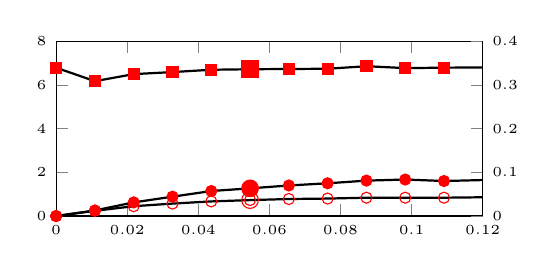
\begin{tikzpicture}
        \begin{axis}[
          %ylabel={Rationing + Repayment},
          ylabel style={font=\tiny, inner sep=0pt, xshift=0pt},
          ymin=0, ymax=8,
          xmin=0, xmax=0.12,
          xticklabel style={/pgf/number format/fixed, /pgf/number format/precision=3},
          width=7cm, height=3.8cm,
          font=\tiny,
        ]
          \addplot[only marks, mark=square*, red] coordinates { (1e-05,6.7931) (0.01091909090909091,6.1768) (0.02182818181818182,6.4994) (0.03273727272727273,6.5926) (0.04364636363636364,6.6995) (0.05455545454545455,6.7234) (0.06546454545454546,6.7342) (0.07637363636363637,6.7453) (0.08728272727272728,6.8621) (0.09819181818181819,6.7748) (0.1091009090909091,6.7942) (0.12001,6.8065) };
          \addplot[black, thick] coordinates { (1e-05,6.7931) (0.01091909090909091,6.1768) (0.02182818181818182,6.4994) (0.03273727272727273,6.5926) (0.04364636363636364,6.6995) (0.05455545454545455,6.7234) (0.06546454545454546,6.7342) (0.07637363636363637,6.7453) (0.08728272727272728,6.8621) (0.09819181818181819,6.7748) (0.1091009090909091,6.7942) (0.12001,6.8065) };
          \addplot[only marks, mark=square*, red, mark size=3pt] coordinates { (0.05455545454545455,6.7234) };
          \addplot[only marks, mark=o, red] coordinates { (1e-05,0.00) (0.01091909090909091,0.24) (0.02182818181818182,0.45) (0.03273727272727273,0.57) (0.04364636363636364,0.67) (0.05455545454545455,0.73) (0.06546454545454546,0.78) (0.07637363636363637,0.80) (0.08728272727272728,0.84) (0.09819181818181819,0.84) (0.1091009090909091,0.84) (0.12001,0.86) };
          \addplot[black, thick] coordinates { (1e-05,0.00) (0.01091909090909091,0.24) (0.02182818181818182,0.45) (0.03273727272727273,0.57) (0.04364636363636364,0.67) (0.05455545454545455,0.73) (0.06546454545454546,0.78) (0.07637363636363637,0.80) (0.08728272727272728,0.84) (0.09819181818181819,0.84) (0.1091009090909091,0.84) (0.12001,0.86) };
          \addplot[only marks, mark=o, red, mark size=3pt] coordinates { (0.05455545454545455,0.73) };
        \end{axis}
        \begin{axis}[
          %ylabel={Contagion},
          ylabel style={font=\tiny, inner sep=0pt, xshift=-5pt},
          ymin=0, ymax=0.4,
          xmin=0, xmax=0.12,
          xticklabel style={/pgf/number format/fixed, /pgf/number format/precision=3},
          axis y line*=right, axis x line=none,
          ylabel near ticks,
          width=7cm, height=3.8cm,
          font=\tiny,
        ]
          \addplot[only marks, mark=*, red] coordinates { (1e-05,0.0000) (0.01091909090909091,0.0128) (0.02182818181818182,0.0313) (0.03273727272727273,0.0443) (0.04364636363636364,0.0573) (0.05455545454545455,0.0634) (0.06546454545454546,0.0700) (0.07637363636363637,0.0750) (0.08728272727272728,0.0811) (0.09819181818181819,0.0836) (0.1091009090909091,0.0802) (0.12001,0.0824) };
          \addplot[black, thick] coordinates { (1e-05,0.0000) (0.01091909090909091,0.0128) (0.02182818181818182,0.0313) (0.03273727272727273,0.0443) (0.04364636363636364,0.0573) (0.05455545454545455,0.0634) (0.06546454545454546,0.0700) (0.07637363636363637,0.0750) (0.08728272727272728,0.0811) (0.09819181818181819,0.0836) (0.1091009090909091,0.0802) (0.12001,0.0824) };
          \addplot[only marks, mark=*, red, mark size=3pt] coordinates { (0.05455545454545455,0.0634) };
        \end{axis}
        \end{tikzpicture}
      \end{figure}
      \vspace{-0.4cm}
      \renewcommand{\arraystretch}{0.55}\setlength{\tabcolsep}{1.2pt}
      \centering
      \tiny
      \begin{tabular}{@{}l@{\hspace{0.15cm}}l@{}}
        \begin{tabular}{lccc}
          \toprule
          $p$ & Rat. & Cont. & Fail. \\
          \midrule
          0.00001 & 6.79 & 0.00 & 0.00 \\
          0.011 & 6.18 & 0.01 & 0.24 \\
          0.022 & 6.50 & 0.03 & 0.45 \\
          0.033 & 6.59 & 0.04 & 0.57 \\
          0.044 & 6.70 & 0.06 & 0.67 \\
           \textbf{0.055} &  \textbf{6.72} &  \textbf{0.06} &  \textbf{0.73} \\
          0.065 & 6.73 & 0.07 & 0.78 \\
          0.076 & 6.75 & 0.07 & 0.80 \\
          0.087 & 6.86 & 0.08 & 0.84 \\
          0.098 & 6.77 & 0.08 & 0.84 \\
          0.109 & 6.79 & 0.08 & 0.84 \\
          0.120 & 6.81 & 0.08 & 0.86 \\
          \bottomrule
        \end{tabular}
        &
        \begin{tabular}{l}
          \textcolor{red}{$\blacksquare$} Rationing \\
          \textcolor{red}{$\circ$} Failed \\
          \textcolor{red}{$\bullet$} Contagion
        \end{tabular}
      \end{tabular}
    \end{column}
  \end{columns}
\end{frame}


%======================================================================
\section{Phase Transition and Results}\label{sec:6}
%======================================================================

\begin{frame}[shrink=0.1]{Phase Transition}
  \begin{itemize}
    \item \textbf{Percolation threshold:} GCS jumps from $\sim 1$ to $\sim 46$ banks ($92\%$).
    \item \textbf{Low $p$:} rationing-dominated, high interest rates, few loans.
    \item \textbf{High $p$:} repayment-failure-dominated, low rates, saturated network.
    \item $p > 0.05$: all macroeconomic metrics stabilize.
  \end{itemize}
\end{frame}

\begin{frame}[shrink=0.1]{Phase Transition}

  \vspace{0.05cm}

  \begin{columns}[T]
    \begin{column}{0.55\textwidth}
      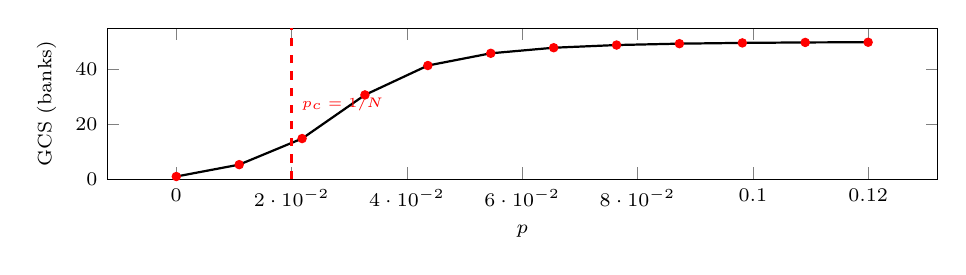
\begin{tikzpicture}
        \begin{axis}[
          width=\textwidth,
          height=3.5cm,
          xlabel={$p$},
          ylabel={GCS (banks)},
          ymin=0, ymax=55,
          font=\scriptsize,
        ]
        \addplot[red, only marks, mark=*, mark size=1.5pt] coordinates {
          (0.00001, 1.01)
          (0.01092, 5.33)
          (0.02183, 14.83)
          (0.03273, 30.72)
          (0.04364, 41.42)
          (0.05455, 45.87)
          (0.06546, 47.90)
          (0.07637, 48.88)
          (0.08727, 49.38)
          (0.09818, 49.66)
          (0.10909, 49.83)
          (0.12000, 49.90)
        };
        \addplot[black, thick] coordinates {
          (0.00001, 1.01)
          (0.01092, 5.33)
          (0.02183, 14.83)
          (0.03273, 30.72)
          (0.04364, 41.42)
          (0.05455, 45.87)
          (0.06546, 47.90)
          (0.07637, 48.88)
          (0.08727, 49.38)
          (0.09818, 49.66)
          (0.10909, 49.83)
          (0.12000, 49.90)
        };
        \draw[red, dashed, thick] (axis cs:0.02,0) -- (axis cs:0.02,55)
          node[pos=0.5, right, font=\tiny]{$p_c = 1/N$};
        \end{axis}
      \end{tikzpicture}
      \vspace{0.1cm}
      \centering
      \textbf{Percolation threshold} for Erd\H{o}s--R\'enyi graph:
      \[
        p_c = \frac{1}{N} = \frac{1}{50} = 0.02
      \]
    \end{column}
    \begin{column}{0.42\textwidth}
      \footnotesize
      \centering
      \begin{tabular}{rr}
        \toprule
        $p$ & GCS \\
        \midrule
        0.00001 & 1 \\
        0.011 & 5 \\
        \textbf{0.022} & \textbf{15} \\
        0.033 & 31 \\
        0.044 & 41 \\
        \textbf{0.055} & \textbf{46} \\
        0.065 & 48 \\
        0.087 & 49 \\
        $\geq 0.11$ & 50 \\
        \bottomrule
      \end{tabular}
    \end{column}
  \end{columns}
\end{frame}


\begin{frame}{Connectivity and Systemic Risk}
  \begin{itemize}
    \item As $p$ increases, the interest rate drops from $30$ (upper bound) to $\sim 1.65$.
    \item Bankruptcies remain stable at $\sim 7$--$7.5$ (limited by model structure).
    \item Active loans saturate at $\sim 13$ ($26\%$ of banks).
    \item Equity jumps from $46.8$ to $\sim 55$ and then plateaus.
    \item Bad debt grows rapidly before stabilizing at $\sim 1.3$.
  \end{itemize}
\end{frame}


%======================================================================
\section{Conclusions}\label{sec:7}
%======================================================================

\begin{frame}{Key Findings}
  As connectivity $p$ increases:
  \begin{enumerate}
    \item The network becomes more connected.
    \item Market power decreases.
    \item The probability of bankruptcy rises.
    \item The equilibrium interest rate falls.
    \item Market power has a greater effect on the interest rate than the probability of bankruptcy does.
    \item Competition mitigates risk more effectively than isolation.
  \end{enumerate}
\end{frame}



\begin{frame}{Key Findings}
  \begin{enumerate}
    \item \textbf{Phase transition at $p \approx 0.05$}: the network saturates and all metrics stabilize.
    \item \textbf{Failure composition shifts}: rationing dominates at low $p$; repayment failure dominates at high $p$.
    \item \textbf{Contagion is minimal} ($<5\%$ of failures)---the dominant risk channel is business failure, not network propagation.
    \item \textbf{Market power} ($\psi$) is positively correlated with rates and decreases as connectivity increases.
  \end{enumerate}
\end{frame}

\begin{frame}{Policy Implications}
  \begin{itemize}
    \item \textbf{Heterogeneity} is a root cause of systemic instability; failure of large banks is catastrophic.
    \item Interbank lending should ideally be restricted among banks with \textbf{similar liquidity characteristics}.
    \item Reserve requirements dampen cascades but \textbf{limit growth}.
    \item Risk diversification across many agents has \textbf{ambiguous} effects on total systemic stability.
  \end{itemize}
\end{frame}

\end{document}
